\section{Inducción matemática, parte II}
Podemos usar inducción matemática para demostrar propiedades numéricas.

%----------------------------------------------------------------------------------------
\subsection{Ejemplo 1}
\begin{itemize}
    \item Demuestre que $1+2+3+...+n = n(n+1)/2$ 
    \item \emph{Prueba}: Por inducción matemática. 
    \item Sea $p(n):=1+2+3+...+n=n(n+1)/2, \forall n \geq 1$. 
\end{itemize}

\underline{Paso base:} Porbar $p(1)$ es verdad.
\begin{center}
   \begin{align*}
       1 = 1(1+1)/2 \\ 
       1 = 1 \\ 
   \end{align*}
\end{center}

\underline{Paso unductivo:} Asumimos $p(k) := 1+2+3+...+k=k(k+1)/2$, para algun $k \geq 1$. (Si se cae el numero k se cae el que sigue).
\begin{center}
   \begin{align*}
       \text{ Demostramos } \qq &p(k+1):= \overbrace{1+2+3+...+k}^{\text{ Hipótesis inductiva }}+(k+1) \\ 
        & p(k+1) :=k(k+1)/2 + k+1 \qq \text{ \# En este punto hacemos uso de la hipótesis inductiva. } \\ 
        & p(k+1):= (k+1)(k/2+1) = (k+1)\overbrace{(k+2)/2}^{k/2+1=(k+2)/2} \\ 
        & p(k+1) := (k+1)((k+1)+1)/2 \qq \text{ \# La proposición es verdadera para $k+1$ también }\\ 
   \end{align*}
\end{center}

En conclusión, la proposición $p(n)$ es verdadera $\forall n \geq 1$  $\square $

%----------------------------------------------------------------------------------------
\subsection{Ejemplo 2}
\begin{itemize}
    \item Demuestre que para todo $n\geq 0$ vale $6^n-1$ es múltiplo de 5. 
    \item Prueba: por inducción matemática. 
    \item Sea $p(n):=6^n-1=5m$, $\forall n \geq 0$ y $m \in Z$.
\end{itemize}

\underline{Paso base:} Probamos $p(0)$. Siempre probamos el primer número.
\begin{center}
   \begin{align*}
       6^0-1 = 0 = 5\times 0 \\ 
   \end{align*}
\end{center} 

\underline{Paso inductivo: } Asumimos $p(k), k \geq 0$, asumir $p(k)$ implica que $p(k):=6^k-1=5m$, donde veamos $p(k)$ podemos usar $5m$.

\begin{center}
   \begin{align*}
    \text{ Demostramos:}\qq & p(k+1):=6^{k+1}-1=5m \\ 
    & p(k+1):= (6\cdot 6^k -6)+5 \\ 
    & p(k+1):= 6\overbrace{(6^k-1)}^{5m}+5 \qq  \text{ \# Hipótesis inductiva } \\ 
    & p(k+1):= 6\cdot 5m + 5 \\ 
    & p(k+1):= 5(6m+1) = 5m_1, \qq \text{ en donde $m_1=6m+1$ } \\ 
   \end{align*}
\end{center}

\underline{En conclusión}, $p(n)$ es verdadera para todo $n\geq 0$ $\square$


%----------------------------------------------------------------------------------------
\subsection{Ejercicio de prueba}
\begin{itemize}
    \item Demuestre que para todo $n\geq 7$ vale la siguiente propiedad $n!>3^n$ 
\end{itemize}

\section{Invariantes e inducción matemática}
\emph{Ejemplo 4}: Supongamos que tenemos un peón que puede moverse en un tablero estándar de ajedrez. El peón comienza en la posición mostrada y en cada paso se mueve hacia arriba o abajo 1 unidad e izquierda o derecha 1 unidad. El peón debe moverse exactamente una unidad en cada dirección (vertical y horizontal). Proponga una estrategia para llevar el peón al punto mostrado en la figura.
\begin{figure}[H]
    \centering
    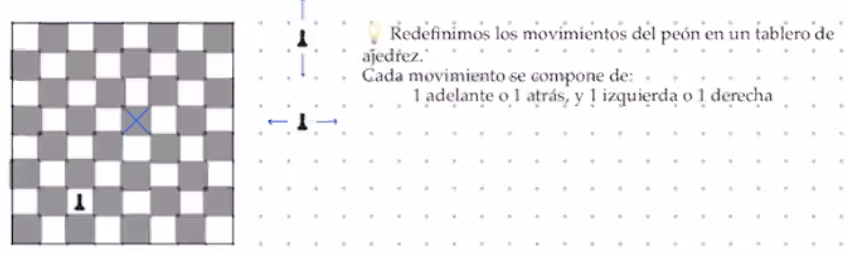
\includegraphics[width=14cm]{\figs/ajedrez} 
\end{figure}
Aparentemente, no es posible llevar al peón hasta la casilla indicada usando los movimientos permitidos, ya que este juego tiene una \emph{propiedad invariante}. \newline 
Una propiedad invariante o simplemente invariantes es una propiedad que permanece inalterada a lo largo de una secuencia de pasos. \newline 

\begin{figure}[H]
    \centering
    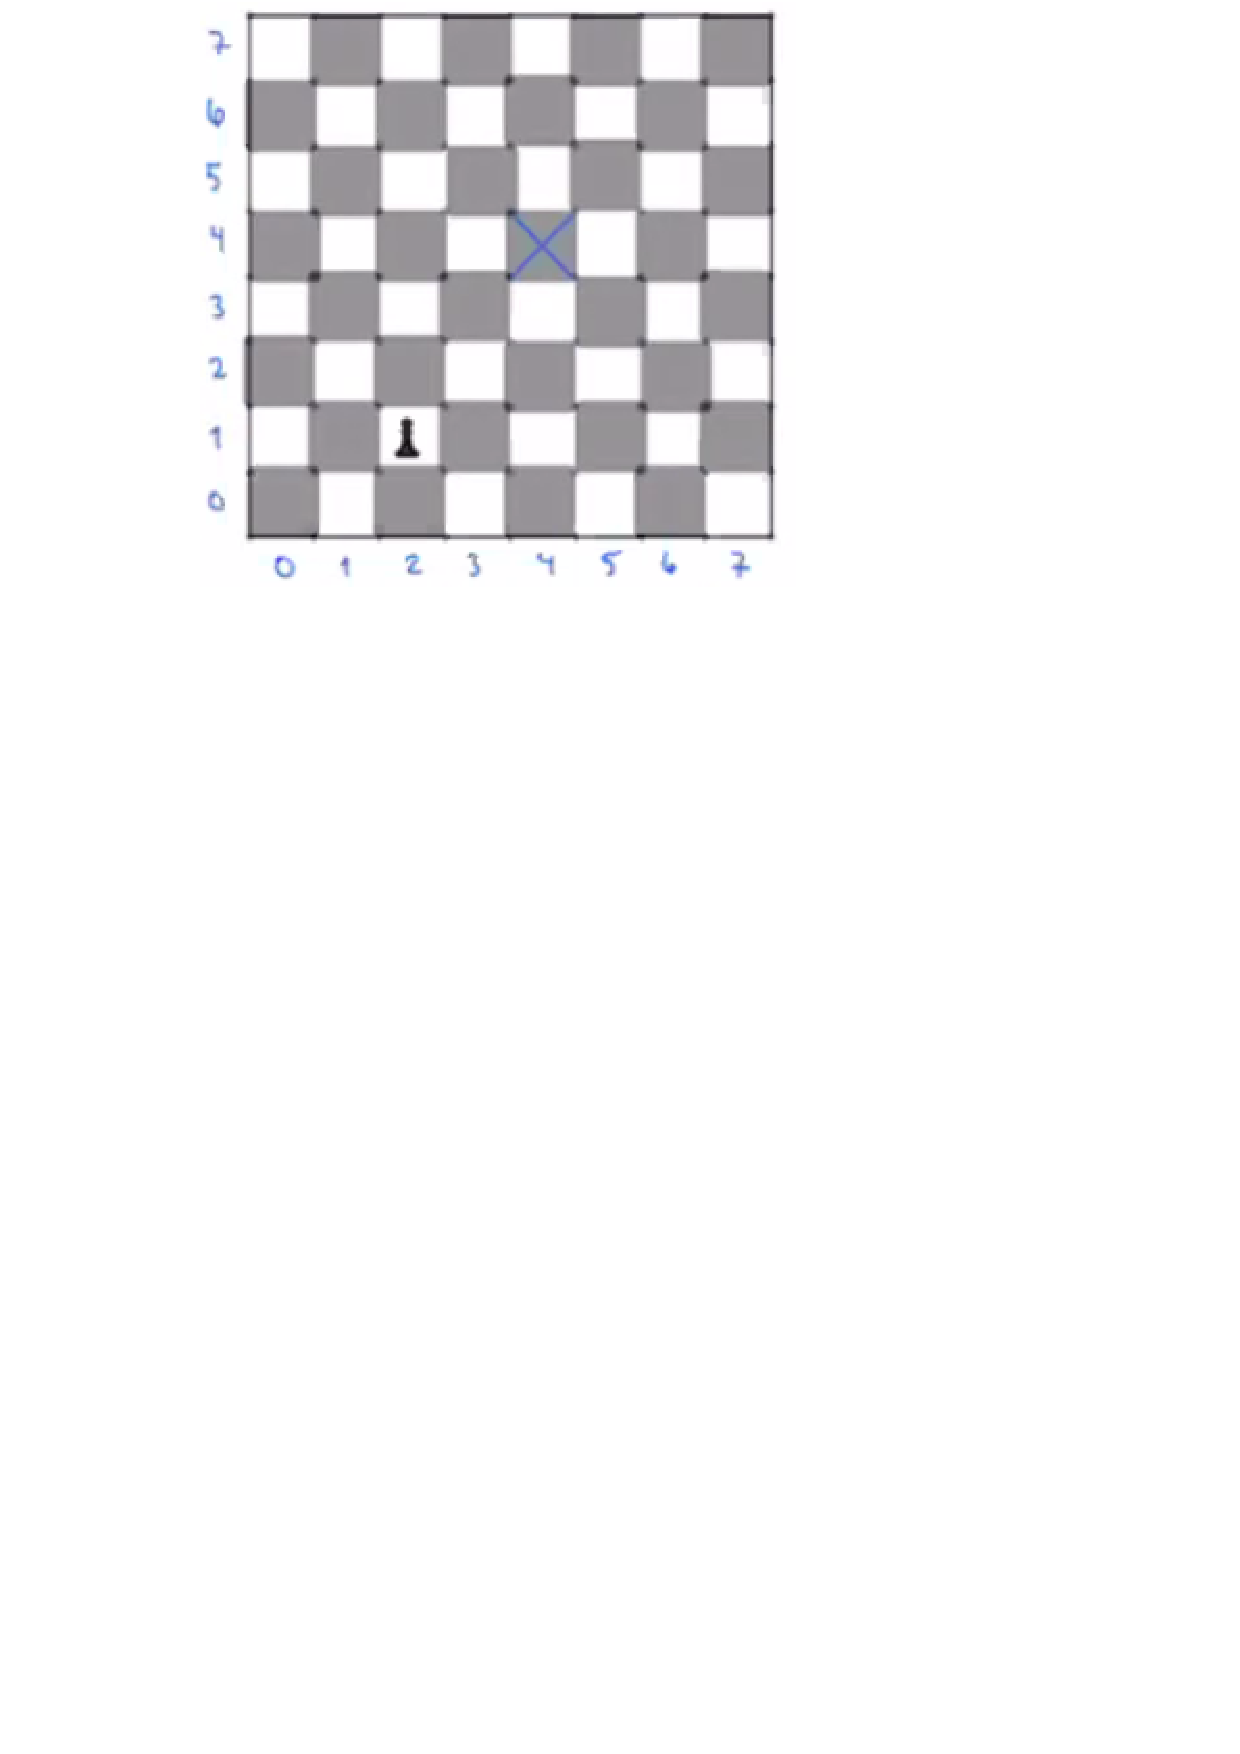
\includegraphics[scale=0.5]{\figs/ajedreznum} 
\end{figure}

Aseguramos que so le llamamos $(x,y)$ a la posición del peón en el tablero, entonces luego de $n$  movimiento permitido se cumplirá que: $x+y$ es impar. \newline 
Esta es la propiedad \emph{invariante del juego}. \newline 

Proposición: Sea $p(n):=$ Luego de $n$ moviemintos, la suma de las coordenadas de la posición del peón es un número impar, i.e, $(x,y)$ la posición, entonces $x+y$ es impar con $n\geq 0$.
\newline 
\underline{Paso base:} Probamos $p(0)$ \newline 
    Luego de 0 movimientos, suposición es $(2,1)$. Luego, $2+1=3$, un número impar. \newline 

\underline{Paso unductivo: } Asumimos $p(k)$, i.e., luego de $k$ movimientos $x*+y*=2m+1$ es impar, en donde $(x*,y*)$ es la posición del peón luego de los $k\geq 0$ movimientos. \newline 

Demostramos $p(k+1)$, i.e., luego de $k+1$ movimientos. Esto lo hacemos por casos. 
COMPONER CASOS.
\begin{itemize}
    \item Caso 1: Derecha y arriba, $(x*,y*)\implies (x*+1,y*+1) \implies x*+1+y*+1 = (2m+1)+2 = 2(m+1)+1 = 2m_1+1$.
    \item Caso 2: Derecha y abajo,  $(x*,y*)\implies (x*+1,y*+1) \implies x*+1+y*+1 = (2m+1)+2 = 2(m+1)+1 = 2m_1+1$.
    \item Caso 3: Izquierda y arriba,  $(x*,y*)\implies (x*-1,y*+1) \implies x*-1+y*+1 = (2m+1)+2 = 2(m+1)+1 = 2m_1+1$.
    \item Caso 4: Izquierda y arriba,  $(x*,y*)\implies (x*-1,y*-1) \implies x*-1+y*-1 = (2m+1)-2 = 2(m-1)+1 = 2m_1+1$.
\end{itemize}

\emph{Corolario:} Como la casilla a la que se pide llegar es $(4,4) \implies 4+4=8$, es un número par, entonces es imposible mover el peón hasta dicha casilla usando los movimientos permitidos. $\square$.
